\documentclass[12pt]{article}
\usepackage[top=1in, bottom=1in, left=.75in, right=.75in]{geometry}
\usepackage{amsmath}



%\usepackage{draftwatermark}
%\SetWatermarkText{draft}
%\SetWatermarkScale{1}
%\SetWatermarkLightness{.9}

\usepackage[]{enumitem}
\usepackage{wrapfig}
%\usepackage{enumerate}
\usepackage{fancyhdr}
%\usepackage{graphicx, xcolor, setspace, adjustbox}
\usepackage{txfonts}
\usepackage{multicol,coordsys,pgfplots}
\usepackage[scaled=0.86]{helvet}
\renewcommand{\emph}[1]{\textsf{\textbf{#1}}}
\usepackage{anyfontsize}
% \usepackage{times}
% \usepackage[lf]{MinionPro}
\usepackage{tikz,pgfplots}
%\def\degC{{}^\circ{\rm C}}
\def\ra{\rightarrow}
\usetikzlibrary{calc,arrows.meta, shapes, angles, quotes}
\pgfplotsset{compat = newest}
\newcommand{\blank}[1]{\rule{#1}{0.75pt}}

\pgfplotsset{my style/.append style={axis x line=middle, axis y line=
middle, xlabel={$x$}, ylabel={$y$}}}


%\usepackage{draftwatermark}
%\SetWatermarkText{Draft}
%\DraftwatermarkOptions{color={[gray]{.9}}}
%\SetWatermarkScale{1.5}

%axis equal

%yticklabels={,,} , xticklabels={,,}

% \setmainfont{Times}
% \def\sansfont{Lucida Grande Bold}
\parindent 0pt
\parskip 4pt
\pagestyle{fancy}
\fancyfoot[C]{\emph{\thepage}}
\fancyfoot[R]{v1}
\fancyhead[L]{\ifnum \value{page} > 1\relax\emph{Math F251X Calculus I: Final Exam}\fi}
\fancyhead[R]{\ifnum \value{page} > 1\relax\emph{Spring 2026}\fi}
\headheight 15pt
\renewcommand{\headrulewidth}{0pt}
\renewcommand{\footrulewidth}{0pt}
\let\ds\displaystyle
\def\continued{{\emph {Continued....}}}
\def\continuing{{\emph {Problem \arabic{probcount} continued....}}\par\vskip 4pt}


\newcounter{probcount}
\newcounter{subprobcount}
\newcounter{subsubprobcount}
\newcommand{\thesubproblem}{\emph{\alph{subprobcount}.}}
\newcommand{\thesubsubproblem}{\emph{\roman{subsubprobcount}.}}
\def\problem#1{\setcounter{subprobcount}{0}%
\addtocounter{probcount}{1}{\emph{\arabic{probcount}.\hskip 1em(#1)}}\par}
\def\subproblem#1{\par\hangindent=1em\hangafter=0{%
\addtocounter{subprobcount}{1}\thesubproblem\emph{#1}\hskip 1em}}
\def\subsubproblem#1{\par\hangindent=1em\hangafter=0{%
\addtocounter{subsubprobcount}{1}\thesubsubproblem\emph{#1}\hskip 1em}}
\def\probskip{\vskip 10pt}
\def\medprobskip{\vskip 2in}
\def\subprobskip{\vskip 45pt}
\def\bigprobskip{\vskip 4in}


\newenvironment{subproblems}
{\begin{enumerate}\renewcommand{\labelenumi}{\emph{\alph{enumi}.}}}
{\end{enumerate}}

\newenvironment{subsubproblems}{%
\begin{enumerate}%
\setcounter{enumi}{\value{subsubprobcount}}%
\renewcommand{\theenumi}{\emph{\roman{enumi}}}}%
{\setcounter{subprobcount}{\value{enumi}}\end{enumerate}}


\newcommand{\be}{\begin{enumerate}}
\newcommand{\ee}{\end{enumerate}}


\begin{document}

{\emph{\fontsize{26}{28}\selectfont Spring 2026 \hfill
\hfill Math F251X}}

\begin{center}
{\emph{\fontsize{32}{36}\selectfont Calculus I: Final Exam}}
\end{center}
\vskip 1.cm

\strut\vtop{\halign{\emph#\hskip 0.5em\hfil&#\hbox to 2in{\hrulefill}\cr
\emph{\fontsize{18}{22}\selectfont Name:}&\cr
\noalign{\vskip 10pt}
%\emph{\fontsize{18}{22}\selectfont Student Id:}&\cr
%\noalign{\vskip 10pt}
%\emph{\fontsize{18}{22}\selectfont Calculator Model:}&\cr
}}
\hfill
\vtop{\halign{\emph{\fontsize{18}{22}\selectfont #}\hfil& \emph{\fontsize{18}{22}\selectfont\hskip 0.5ex $\square$ #}\hfil\cr
Section: & 9:15 (James Gossell)\cr
\noalign{\vskip 4pt}
         & 11:45 (Gordon Williams)\cr
\noalign{\vskip 4pt}
         & Online (James Gossell)\cr}}
%
%\vfill


{\fontsize{16}{18}\selectfont\emph{Rules:}}
\begin{itemize}
\item Partial credit will be awarded, but you must {\bf show your work}.

\item You may have a single handwritten $3'' \times 5''$ notecard, both sides.

\item Personal calculators are \emph{not allowed}. 

\item Place a box around your  \fbox{FINAL ANSWER} to each question where appropriate.

\item Turn off anything that might go beep during the exam.

\item You have two hours to complete the exam.

\end{itemize}


%If you need extra space, you can use the back sides of the pages.
%Please make it obvious  when you have done so.

%Good luck!
%\vfill
\def\emptybox{\hbox to 2em{\vrule height 16pt depth 8pt width 0pt\hfil}}
\def\tline{\noalign{\hrule}}
\centerline{\vbox{\offinterlineskip
{
\bf\sf\fontsize{18pt}{22pt}\selectfont
\hrule
\halign{
\vrule#&\strut\quad\hfil#\hfil\quad&\vrule#&\quad\hfil#\hfil\quad
&\vrule#&\quad\hfil#\hfil\quad&\vrule#\cr
height 3pt&\omit&&\omit&&\omit&\cr
&Problem&&Possible&&Score&\cr\tline
height 3pt&\omit&&\omit&&\omit&\cr
&1&&9&&\emptybox&\cr\tline
&2&&9&&\emptybox&\cr\tline
&3&&12&&\emptybox&\cr\tline
&4&&12&&\emptybox&\cr\tline
&5&&10&&\emptybox&\cr\tline
&6&&10&&\emptybox&\cr\tline
&7&&10&&\emptybox&\cr\tline
&8&&14&&\emptybox&\cr\tline
&9&&14&&\emptybox&\cr\tline 
%&11&&?&&\emptybox&\cr\tline \tline 
&Extra Credit&&(5)&&\emptybox&\cr\tline \hline
&Total&&100&&\emptybox&\cr
}\hrule}}}



\newpage



%Compute Limits
\problem{9 points} Compute the following \emph{limits}. Show your work clearly. Make sure you use \emph{limit notation} where required and not where it isn't; an answer that does not use proper notation will not receive full credit. Use = to show things are equal. If you use L'H\^opital's rule, write $\stackrel{H}{=}$ or  $\stackrel{L'H}{=}$ to indicate where you are applying it.
\begin{subproblems}
\item $\displaystyle\lim_{x\to\infty} \frac{3x^2+3e^{-2x}}{x^{2}-e^{-x}}$
\vfill
\item $\displaystyle\lim_{t\to 1^{+}}\frac{(t+1)(t+2)}{1-t^{2}}$
\vfill
\item  $\displaystyle\lim_{h\to 0}\frac{6xh-3h^{2}+h}{h}$
\vfill
\end{subproblems}



\newpage



%Compute derivatives
\problem{9 points} Compute the following derivatives. Simplify your answers.
\begin{subproblems}
\item $\displaystyle\frac{d}{dx} \ln(3x)\sec(2x)$
\vfill
\item $\displaystyle\frac{d}{dt} \frac{{t+1}}{t-2}$
\vfill
\item $\displaystyle\frac{d}{dt} \sin(\cos^{2}(3t)+t)$
\vfill
\end{subproblems}



\newpage



%Compute Integrals
\problem{12 points} Compute the following \emph{integrals}. Give the most general answer, and show your work. Clearly indicate any substitutions you use in such a way that someone else can follow your work. Do not put a $+C$ where it does not belong, and you must include $+C$ where it is needed.



\begin{subproblems}
	\item  $\displaystyle\int_{1}^{3}10x^{4}-12x^{2}\: dx $
	\vfill
	\item $\displaystyle \int_{-2}^{2}\frac{2x+3}{(2x^{2}+6x)^{2/3}}\: dx  $
	\vfill
	\item $\displaystyle\int \frac{2x}{\sqrt{1-x^{4}}}\: dx$
	\vfill
	\item $\displaystyle \int xe^{3x^{2}}\: dx$
	\vfill
\end{subproblems}



\newpage



%Sketch graph
\problem{12 Points} \emph{Sketch} a graph of a function $f(x)$ that satisfies all of the following properties.

After drawing the graph:
\begin{itemize}
\item \emph{Label} on the graph the following things, if they exist, by drawing a point on the graph and labeling: any local maximums by writing  \textsf{LOCAL MAX}, local minimums by writing \textsf{LOCAL MIN}, inflection points by writing \textsf{IP} 
\item Draw any horizontal and vertical asymptotes with dashed lines and \emph{label} them with their equation.
\item Mark any important $x$-values and $y$-values on the $x$- and $y$-axes.
\end{itemize}

\emph{Properties:}

\begin{multicols}{2}
\begin{itemize}[noitemsep, topsep=0pt]
\item The domain of $f(x)$ is $(-\infty, 2)\cup(2, \infty)$\\
\item $f(-2)=0$\\
\item $f(0)=-2$\\
\item $\ds{\lim_{x \to \infty} f(x) = 0}$\\
\item $\ds{\lim_{x \to -\infty} f(x) = 2}$\\
\columnbreak
\item $\ds{\lim_{x \to 2^+} f(x) = -\infty}$\\
\item $f'(x) > 0$ on $(0,2)\cup(2,\infty)$\\
\item $f'(x) < 0$ on $(-\infty,0)$\\
\item $f''(x) > 0$ on $(-2, 2)$\\
\item $f''(x) <0$ on $(\infty,-2)\cup(2,\infty)$\\
\end{itemize}
\end{multicols}


\begin{tikzpicture}
\draw[<->] (-8,0) --  (8,0);
\draw[<->] (0,5) -- (0,-5);
\end{tikzpicture}



\newpage



%Optimization
\problem{10 Points} %Optimization
You have 900 m of fencing to make a rectangular pen for llamas, with one side of the pen abutting a river (so no fence needed on that side). What are the dimensions of the pen that maximizes the enclosed area? \emph{Include units.} Fully justify your conclusions.

\hfill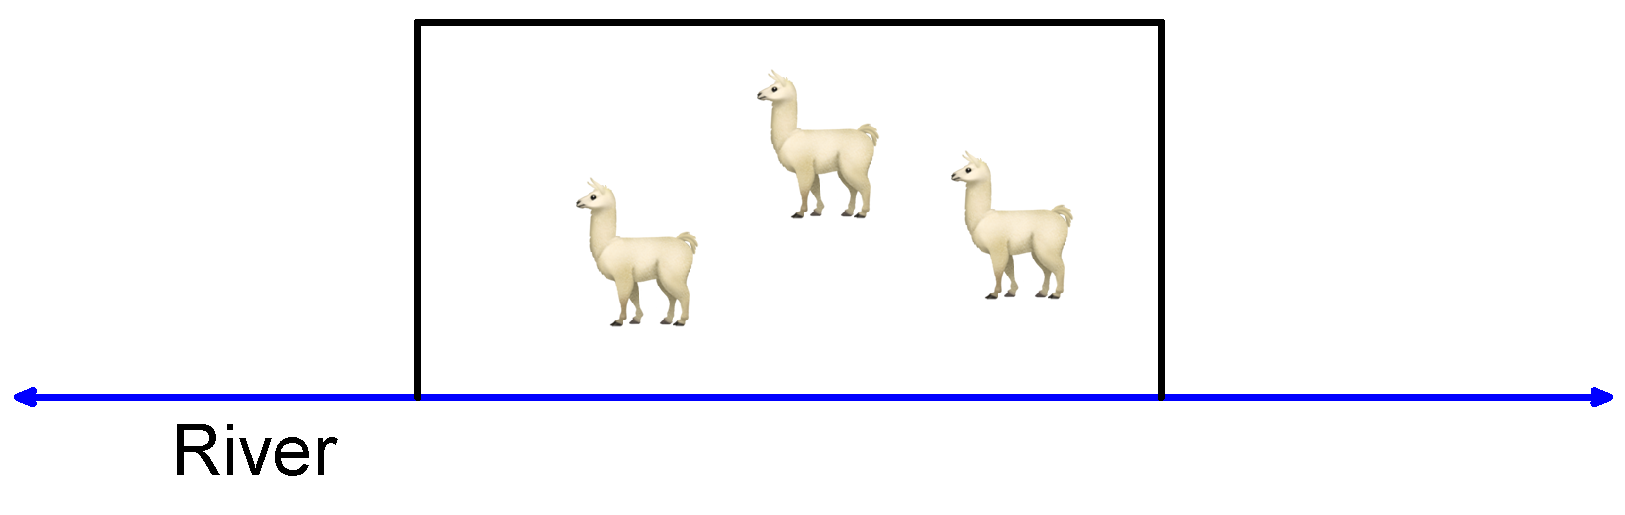
\includegraphics[width=5in]{River}



\newpage



%Identify things from a graph
\problem{10 points} 

The graph of a function $g(x)$ is shown below. Use the graph to answer each question below. If the value does not exist or is undefined, write {\sf DNE}.\\

\newcommand{\ans}{\rule{1cm}{.5pt}}

\begin{center}
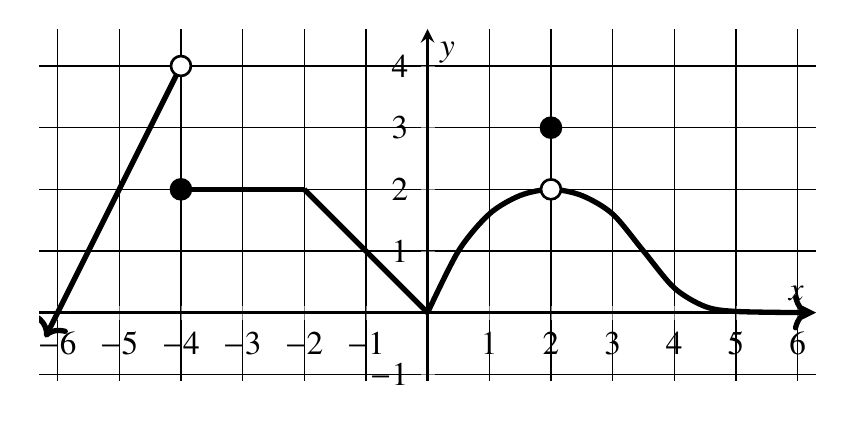
\begin{tikzpicture}[scale = 1.2]
\begin{axis}[scale=1.2, thick, my style, xtick={-6,-5,-4,...,6}, ytick={-1,1,2,...,4},
xmin=-6.3, xmax=6.3, ymin=-1.1, ymax=4.6, minor y tick num=0,
        minor x tick num=0, mark size=3.0pt, grid=both, grid style={ thin, black, %dashed
        }, axis equal image]
% %%asymptote
\addplot[mark=*,only marks] coordinates {(-4,2)(2,3)};
%%points open
\addplot[mark=*,fill=white,only marks] coordinates {(-4,4)(2,2)};
%%Curves
\addplot[ultra thick,<-] coordinates {(-6.2,-0.4)(-4,4)};
\addplot[ultra thick] coordinates {(-4,2)(-2,2)};
\addplot[ultra thick] coordinates {(-2,2)(0,0)};
\addplot[ultra thick, smooth,->] coordinates {(0,0)(0.5,1)(1,1.6)(1.5,1.9)(2,2)(2.5,1.9)(3,1.6)(3.5,1)(4,0.4)(4.5,0.1)(5,0.02)(6.2,0.0)};

\end{axis}

\end{tikzpicture}
\end{center}

\begin{subproblems}

\begingroup
\setlength{\parskip}{2.5em}
\setlength{\columnsep}{1 cm}
\begin{multicols}{3}
\item $g'(-5)$ = \ans

\item $\ds{\lim_{ x\to-4^{-}}g(x)}$ = \ans

\item $\ds{\lim_{x\to-4}g(x)}$ = \ans

\columnbreak

\item $g'(-3)$ = \ans

\item $\ds\int_{-4}^{0} g(x)$ = \ans% worth 1 point

\item $\ds{\lim_{x\to -2^{+}}g(x)}$ = \ans

\columnbreak

\item $\ds{\lim_{x\to -2^{+}}g'(x)}$ = \ans

\item $\ds{\lim_{x\to 2}g(x)}$ = \ans

\item $\ds{\lim_{x\to \infty}g(x)}$ = \ans

\end{multicols}

\endgroup

\bigskip

\item List all \emph{$\mathbf{x}$-values} in the set $(-6, 6)$ where the function $g(x)$ is \emph{not} continuous. Classify the discontinuity as {\bf infinite}, {\bf jump}, {\bf removable}, or {\bf other}.\\
 
$x = $ \ \hrulefill

\bigskip

\item List all \emph{$\mathbf{x}$-values} in the set $(-6, 6)$ where the function $g(x)$ is \emph{not} differentiable.\\
 
$x = $ \ \hrulefill

\bigskip

\begin{multicols}{2}

\item Is $g''(1)$ positive, negative, or zero?

\columnbreak

\item Is $g''(4)$ positive, negative, or zero?

\end{multicols}

\end{subproblems}



\newpage



%Related rates/implicit differentiation, pythagorean Theorem
\problem{10 Points} 
A painter is using a roller brush at the end of a 15 foot long pole to paint the wall of a building. Suppose the painter is moving towards the wall at a rate of $\frac{1}{2}$ ft/sec. When the painter is 9 feet from the wall, how fast is the brush head moving? Clearly identify whether the brush head is moving up or down. \emph{Include units and simplify your answer}.

\hfill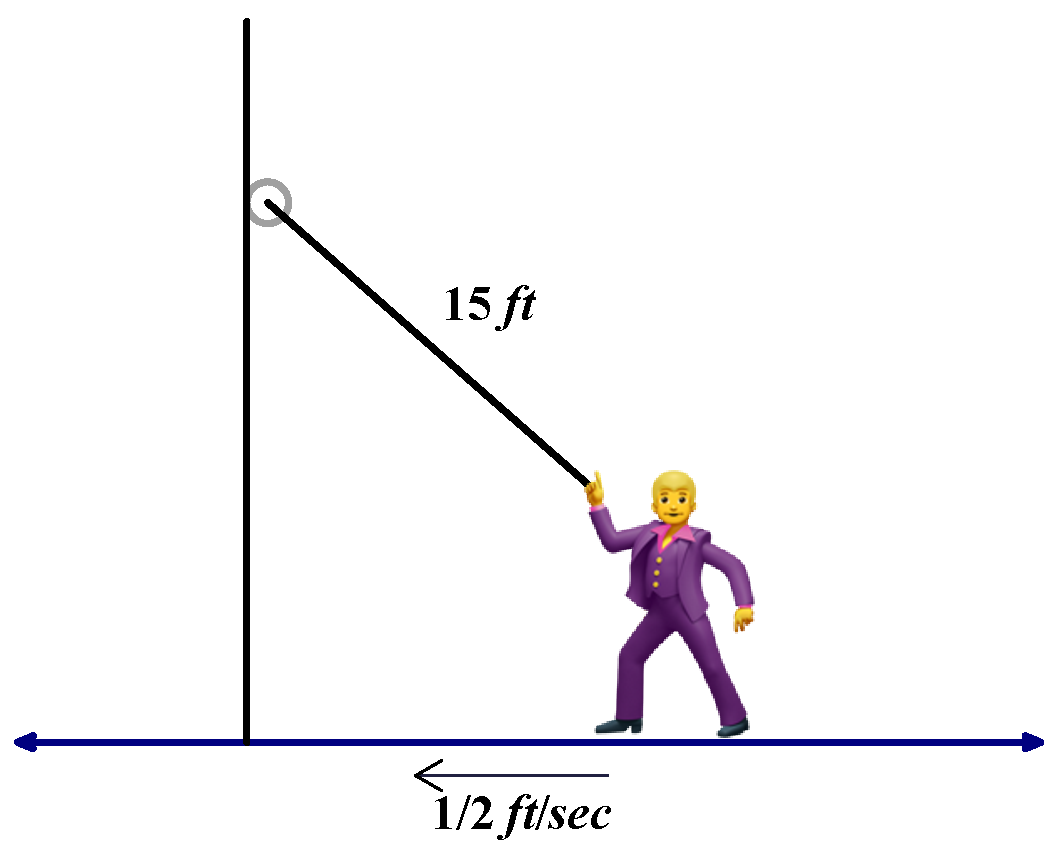
\includegraphics[width=3in]{Painter.pdf}
%%%%%%%%%%% 


\newpage
\problem{14 Points} %1st and 2nd derivative tests
Let $f(x)=3x^{4}-4x^{3}$. 
\begin{subproblems}
\item Find the locations of any local maxima or minima of $f(x)$ on $(-\infty,\infty)$.
\vfill 

\vspace{1cm}
\item Find the absolute maximum and minimum of $f(x)$ on $[-1,2]$.
\vfill
\item On what intervals is $f(x)$ concave up on $(-\infty,\infty)$? On what intervals is $f(x)$ concave down on $(-\infty,\infty)$? If no such an interval exists, say so, and justify your answer.
\vfill
\item What are the locations ($x$-values) of any inflection points of $f(x)$ on $(-\infty,\infty)$? If there are none, say they do not exist and justify your conclusion.
\vspace{.75in}
\end{subproblems}



\newpage



%Velocity, position, acceleration
\problem{14 points} A $4$-story Foucault pendulum assumes small oscillations so that the motion is approximately simple harmonic. The {\bf horizontal velocity} of the pendulum bob is given by:

$$v(t)=-\frac{9}{20}\sin\left(\frac{9}{10}t\right) \text{  meters per second}$$

At time $t=0$ seconds, the pendulum is at its maximum displacement of $0.5$ meters from equilibrium.
\begin{subproblems}

\item Find the horizontal position function $x(t)$ of the pendulum bob at $t$ seconds.
\vfill
\vfill
\item Write a sentence interpreting the meaning of the value of $\displaystyle \int_0^5 v(t) \, dt$ in the context of the problem. {\bf Include units}. {\bf Do not solve}.
\vfill
\item Find the acceleration function $a(t)$ of the pendulum bob at $t$ seconds.
\vfill
\item Evaluate $a(1)$. You do not need to simplify your answer, but you do need to {\bf include units}.
\vfill
\item After $1$ second, is the pendulum bob speeding up or slowing down? Explain your reasoning.\\

(Hint: $\sin(9/10)$ and $\cos(9/10)$ are both positive.)
\vfill
\end{subproblems}




\newpage




%%%%%% 
\problem{Extra Credit: 5 Points}
\begin{wrapfigure}{r}{0.4\textwidth}\centering
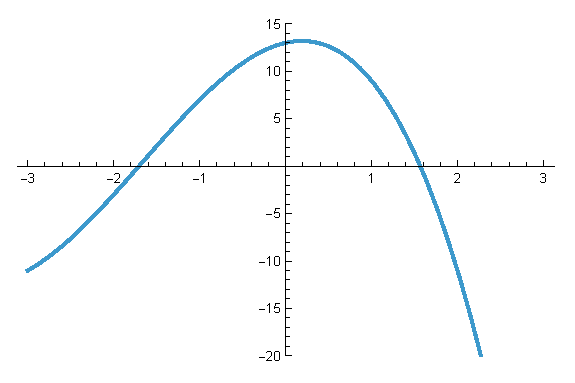
\includegraphics[width=\linewidth]{Newton}
\end{wrapfigure}In this problem you will use Newton's method to estimate the value of a root of a function \[f(x)=-x^3-2 x^2+9 x+7,\] whose graph is given at right.
\begin{subproblems}
\item Describe, in words, how Newton's method works; in other words, what is the main idea of Newton's method? Draw the first step on the graph showing how to obtain $x_{1}$ from $x_{0}=0$.
\vfill
\item Will Newton's method obtain a good estimate for the {\bf positive} root of $f(x)$ starting with $x_{0}=0$? Explain your answer.
\vfill
\item Suppose I start my attempt to find the positive root of $f(x)$ with $x_{0}=2$. What is $x_{1}$? What is $x_{2}$?
\vfill
$x_1=$
\vfill
$x_2=$
\vspace{.3in}
\end{subproblems}


\end{document}

%%%%ENDDOCUMENT
